% =====================================================================
% Fully Symmetry-Conditioned Rigid-Body Flow Matching for
% Molecular-Crystal Structure Prediction
%
% AI4Mat @ NeurIPS 2026 workshop paper (Aug 30). Non-archival, simultaneous
% submission permitted (co-submitted to MoML, Sep 1). Content is identical to the
% MoML short paper (paper/submissions/MoML/main.tex); this copy is kept separate
% so each venue's formatting can diverge.
% Self-contained: compiles with pdflatex + bibtex (natbib) as-is.
% NOTE: convert to the official AI4Mat/NeurIPS style at submission (see
% SUBMISSION_NOTES.md); needs one Overleaf compile pass (no local TeX).
% =====================================================================
\documentclass[10pt]{article}

\usepackage[margin=0.85in]{geometry}
\usepackage{amsmath,amssymb}
\usepackage{graphicx}
\usepackage{booktabs}
\usepackage{microtype}
\usepackage[numbers,sort&compress]{natbib}
\usepackage[colorlinks=true,allcolors=blue]{hyperref}
\usepackage{authblk}
\usepackage{tikz}
\usetikzlibrary{arrows.meta,positioning,fit,backgrounds}
\usepackage{pgfplots}
\pgfplotsset{compat=1.17}

\setlength{\parskip}{0.15em}
\renewcommand{\abstractname}{\vspace{-\baselineskip}}

\title{\bfseries Fully Symmetry-Conditioned Rigid-Body Flow Matching for
Molecular-Crystal Structure Prediction}

\author[1]{Frank Cai\thanks{\texttt{frankyc11223@gmail.com};
ORCID \href{https://orcid.org/0009-0003-0041-1459}{0009-0003-0041-1459}}}
\affil[1]{Purdue University, West Lafayette, IN, USA}
\date{}

\begin{document}
\maketitle

\begin{abstract}
\noindent
Rigid-body flow matching is an efficient route to molecular-crystal structure
prediction, reducing a crystal to a lattice, fractional centroids, and
per-molecule orientations on $\mathrm{SO}(3)$. Recent rigid-body
molecular-crystal flows leave space-group symmetry unconditioned, and
symmetry-conditioned generation has so far been demonstrated only for inorganic
atomic sites, never for rigid-body molecular orientation. We show that the
per-molecule orientation target decomposes as
$R_m=\mathrm{rot}(g_m)\,R_{\text{asym}}$ into a space-group-determined relative
rotation, which a flow can learn, and a gauge-free asymmetric-unit pose, which it
cannot regress from packing. We turn this into a deployable method: a
\emph{leak-free} coset label---the generating space-group operation, recoverable
from a template at sampling time---conditions the orientation flow. On $1{,}127$
crystals from the Cambridge Structural Database, deployable coset conditioning
lifts the held-out non-reference orientation loss by $41.1\%$ (versus $27.5\%$
for a paired no-coset control), recovering two-thirds of the way to a
leaky-codebook oracle ($\sim\!48\%$); an $\mathrm{SO}(3)$-averaged training
objective closes the remaining gap ($47.7\%$). A packing-only predictor recovers
the coset at $39.5\%$ accuracy ($4\times$ the majority baseline) but is not yet
accurate enough for template-free use, which we identify as the key remaining
gap. Extending symmetry conditioning from the orientation to the \emph{lattice} (a
crystal-family mask on a log-metric parametrization) gives, to our knowledge, the
first \emph{fully symmetry-conditioned} molecular-crystal flow; composed with an
unsupervised symmetry-preserving packing finisher and a fully-ablated lever stack,
it lifts held-out exact match from $0\%$ to $6.9\%$ (strict best-of-$10$,
$\text{stol}\,1.0$)---parity with the symmetry-free MolCrystalFlow ($\sim\!8\%$)---and
$10.7\%$ with orientation test-time augmentation (Section~\ref{sec:ladder}).
\end{abstract}

% =====================================================================
\section{Introduction}
% =====================================================================
Crystal structure prediction (CSP) asks for the stable periodic arrangement of a
chemical system. Generative models have become a fast alternative to large
ensembles of density-functional relaxations, progressing from crystal diffusion
autoencoders\cite{xie2022cdvae} to joint equivariant diffusion\cite{jiao2023diffcsp}
and Riemannian flow matching\cite{miller2024flowmm,lipman2023flowmatching,chen2024riemannian},
which learns a straight conditional path solvable in tens of steps.
\emph{Rigid-body} factorization is especially attractive for molecular crystals:
freezing each molecule's conformer collapses dozens of atomic coordinates to a
single pose---a lattice $L$, a fractional centroid $c_m\in\mathbb{T}^3$, and an
orientation $R_m\in\mathrm{SO}(3)$ per molecule---and supports the short sampling
trajectories characteristic of flow matching.

This introduces a per-molecule orientation variable on $\mathrm{SO}(3)$, and here
the current generation of models leaves value on the table. MolCrystalFlow, a
2026 rigid-body molecular-crystal flow with the same
$\text{lattice}\times\mathbb{T}^3\times\mathrm{SO}(3)$ factorization, jointly
learns pose but \emph{does not impose space-group
constraints}\cite{zeng2026molcrystalflow}; MOFFlow likewise flows rigid
$\mathrm{SE}(3)$ poses without a symmetry prior, relying on framework
connectivity to constrain orientation\cite{kim2025mofflow}. Symmetry- and
Wyckoff-conditioned generation, meanwhile, is proven only for
\emph{inorganic atomic sites}: DiffCSP++\cite{jiao2024diffcsppp},
WyckoffDiff\cite{wyckoffdiff2025}, SymmCD\cite{symmcd2025}, and the 2026
NextCrystal\cite{mu2026nextcrystal} all condition atom generation on a
space-group/Wyckoff template, but none touches rigid-body molecular pose. The
gap is precise: nobody has conditioned a rigid-body \emph{molecular orientation}
flow on the crystal's symmetry.

We close that gap. The starting point is a decomposition of the orientation
target, $R_m=\mathrm{rot}(g_m)\,R_{\text{asym}}$, into a space-group-determined
relative rotation between symmetry copies and the asymmetric unit's gauge-free
pose. Classical molecular-CSP codes never search the relative rotation---they
generate symmetry copies by applying space-group
operators\cite{price2023blindtest7,obrien2021dataefficient}---and we find a
learned flow mirrors that division of labor: the relative part is learnable and
the free part is not. The contribution of this paper is to make the learnable
part \emph{deployable}. Our contributions are:
\begin{itemize}\itemsep0.05em
\item A \textbf{leak-free, template-available coset label}---the generating
space-group operation $h=g_m g_0^{-1}$, recovered from centroids alone---that
supplies the symmetry-relative rotation at sampling time without seeing the
target (Section~\ref{sec:coset}), in contrast to a codebook clustered from the
target itself.
\item A coset-conditioned orientation flow and sampler that \textbf{recover
two-thirds of the oracle-codebook benefit} ($+41.1\%$ vs a $+27.5\%$ paired
control on held-out non-reference orientation loss; Section~\ref{sec:gate}).
\item An \textbf{$\mathrm{SO}(3)$-averaged training objective}\cite{cao2025so3averaged}
that closes the remaining gap to the leaky ceiling ($+47.7\%$).
\item A \textbf{packing-only coset predictor} for template-free use ($39.5\%$
top-1, $4\times$ majority) and an honest characterization of the remaining
de-novo gap.
\item The \textbf{first fully symmetry-conditioned molecular-crystal flow}
(orientation coset $\times$ crystal-family lattice mask) and an unsupervised
symmetry-preserving finisher, whose fully-ablated lever stack lifts exact match
from $0\%$ to parity with MolCrystalFlow ($6.9\%$ strict, $10.7\%$ with
orientation TTA; Section~\ref{sec:ladder}).
\end{itemize}

% =====================================================================
\section{Method}
% =====================================================================
\paragraph{Rigid-body flow.}
SymMC-Flow represents a molecular crystal by a lattice
$L\in\mathbb{R}^{3\times3}$ and, per molecule $m$, a fractional centroid
$c_m\in\mathbb{T}^3$ and orientation $R_m\in\mathrm{SO}(3)$ acting on a shared
body-frame conformer, so
$\text{cart}_{m,a}=c_mL+R_m\,\text{local}_{m,a}$. A conditional flow-matching
objective\cite{lipman2023flowmatching} is trained jointly over three manifolds
(a Euclidean path for a volume-normalized lattice, a torus geodesic for
centroids, an $\mathrm{SO}(3)$ geodesic for orientations), with the velocity
field conditioned on the space group. An $\mathrm{E}(n)$-equivariant
encoder\cite{satorras2021egnn} embeds the conformer and pair-bias attention mixes
molecules within the cell (Appendix~\ref{app:method}).

\paragraph{The orientation decomposition.}
A molecule $m$ generated from the asymmetric unit by an operation with rotation
part $\mathrm{rot}(g_m)$ has absolute pose
$R_m=\mathrm{rot}(g_m)\,R_{\text{asym}}$, where $R_{\text{asym}}$ is the free
orientation of the asymmetric unit. Because the body-frame gauge is arbitrary,
$R_{\text{asym}}$ carries no consistent signal tied to composition or packing:
trained directly, the absolute orientation head never beats its predict-zero
floor ($\mathbb{E}\lVert u_R\rVert^2\!\approx\!5.24$), while lattice and centroid
heads converge normally. Re-gauging each crystal so the first copy of a species
is a reference ($R{=}I$) and the others carry only the relative rotation
$R'_m=R_mR_0^{-1}$ cancels $R_{\text{asym}}$ and exposes the learnable factor;
the held-out non-reference loss then drops by $27\%$. This much is a diagnostic;
the rest of the paper makes it a method.

\paragraph{Deployable symmetry-coset conditioning.}
\label{sec:coset}
Within a space group the non-reference relative rotations fall into a small
discrete set of \emph{cosets}: $R'_m$ equals the rotation part of the operation
$h=g_mg_0^{-1}$ that maps the reference copy to copy $m$. We assign each molecule
this generating operation directly from the crystallography---by matching its
fractional centroid against $W_h\,c_0+t_h$ (minimum image) over the space
group's operations $\{(W_h,t_h)\}$ obtained from pymatgen---never from the
observed rotation. The resulting label is \textbf{leak-free} and available at
sampling time from a symmetry template, exactly as DiffCSP++/WyckoffDiff-style
generators supply Wyckoff templates for atoms\cite{jiao2024diffcsppp,wyckoffdiff2025}.
This yields $238$ operation-cosets across the corpus (versus $707$ for a codebook
clustered from the target rotations, whose index is derived in part from the
answer and therefore serves only as an upper bound). The coset index enters the
network as a per-molecule embedding and is threaded through the sampler, so it
conditions both training and generation.

\paragraph{$\mathrm{SO}(3)$-averaged objective.}
The $\mathrm{SO}(3)$ flow-matching residual has high variance because the prior
rotation is drawn uniformly. Following the SO(3)-averaged flow objective for
conformer generation\cite{cao2025so3averaged}, we average the orientation
residual over $K$ prior draws per molecule before the gradient step, reducing
target variance at fixed data.

\paragraph{Packing-only predictor.}
For template-free deployment the coset must be inferred. We train a classifier
that predicts each molecule's coset from the conformer, centroid, lattice, and
space group---\emph{without} orientation, so it cannot leak the target---and use
its prediction in place of the template at sampling time.

\paragraph{Full symmetry conditioning and finishing.}
The coset conditions orientation; the lattice is still free, and an unconstrained
$9$-DOF shape head recovers the crystal family poorly ($16\%$ of cell angles at
$90^\circ$ vs.\ a reference $74\%$). Following DiffCSP++\cite{jiao2024diffcsppp} we
condition the lattice on the crystal family: represent the cell by the
$\mathrm{O}(3)$-invariant log-metric $\log(L^\top L)\in\mathbb{R}^6$ and apply a
binary family mask that freezes the constrained coordinates to canonical values
(after each sampler step and in the prior). This gives a fully symmetry-conditioned
flow, but restoring family geometry ($90^\circ$ angles $16\%\!\to\!74\%$) does not
by itself move exact match---the residual blocker is close-packing precision. We
add an unsupervised, symmetry- and rigidity-preserving \emph{rigid-press finisher}
(a Lennard-Jones relaxation over intermolecular atom pairs, optimizing the
asymmetric-unit pose and the family-masked cell, with symmetry copies regenerated
from the space-group operations each step, never seeing the target), plus a learned
centroid prior, self-conditioning, and AlphaFold-style recycling, each ablated in
Section~\ref{sec:ladder}.

% =====================================================================
\section{Experiments}
% =====================================================================
\paragraph{Setup.}
The corpus is a seeded CSD sample\cite{groom2016csd}: $1{,}127$ ordered organic
molecular crystals, $5{,}048$ rigid blocks, a fixed $964/131$ split, with
$1{,}095$ crystals containing $\ge2$ copies of a species (the multi-copy subset
where a relative target exists). The primary metric is the \emph{held-out
non-reference orientation-loss drop} (percentage reduction from untrained to
trained on non-reference copies, which cannot be earned by predicting the
identity); we also report orientation-isolated StructureMatcher\cite{ong2013pymatgen}
reconstruction (true lattice/centroid/conformer, only $\mathrm{SO}(3)$ sampled,
best of eight draws, following match-rate cautions\cite{martirossyan2025matching}).
All numbers are means over three seeds.

\paragraph{Deployable coset conditioning recovers most of the oracle benefit.}
\label{sec:gate}
Table~\ref{tab:gate} and Fig.~\ref{fig:gate} give the main result. A paired
no-coset control reproduces the $+27.5\%$ baseline. Supplying the deployable,
leak-free coset raises the non-reference drop to $+41.1\%$---recovering about
two-thirds of the way from the baseline to the $\sim\!48\%$ reached by the leaky
codebook that peeks at the target. Adding the $\mathrm{SO}(3)$-averaged objective
($K{=}4$) reaches $+47.7\%$, statistically level with the leaky ceiling. In other
words, the benefit that a target-derived codebook could only \emph{upper-bound}
is realized here by a label a sampler actually has.

\begin{table}[t]
\centering
\caption{Held-out non-reference orientation-loss drop (untrained$\to$trained),
mean$\pm$s.d.\ over three seeds. The deployable coset is leak-free and available
from a template; the leaky codebook (index clustered from the target) is an
upper bound. Deployable conditioning recovers two-thirds of the gap; the
$\mathrm{SO}(3)$-averaged objective closes it.}
\label{tab:gate}
\begin{tabular}{lcc}
\toprule
configuration & non-ref.\ loss drop & deployable? \\
\midrule
no-coset control (baseline)         & $27.5\pm2.7\%$ & --- \\
deployable coset ($K{=}1$)          & $41.1\pm3.4\%$ & yes \\
\quad + $\mathrm{SO}(3)$-averaged ($K{=}4$) & $47.7\pm3.9\%$ & yes \\
leaky codebook (oracle upper bound) & $\sim48\%$      & no  \\
\bottomrule
\end{tabular}
\end{table}

\begin{figure}[t]
\centering
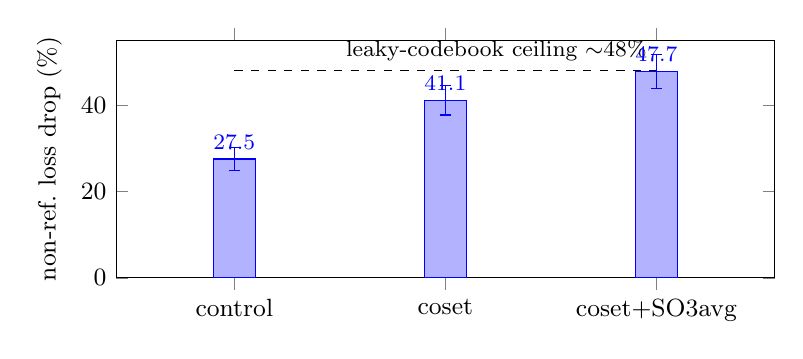
\begin{tikzpicture}
\begin{axis}[
  width=0.82\linewidth, height=4.6cm,
  ybar, bar width=15pt,
  symbolic x coords={control, coset, coset+SO3avg},
  xtick=data, ymin=0, ymax=55,
  ylabel={non-ref.\ loss drop (\%)},
  ylabel style={font=\small}, tick label style={font=\small},
  nodes near coords, nodes near coords style={font=\footnotesize},
  enlarge x limits=0.28,
]
\addplot+[error bars/.cd, y dir=both, y explicit] coordinates {
  (control,27.5) +- (0,2.7)
  (coset,41.1)   +- (0,3.4)
  (coset+SO3avg,47.7) +- (0,3.9)
};
\draw[dashed] (axis cs:control,48) -- (axis cs:coset+SO3avg,48)
  node[above left,font=\footnotesize] {leaky-codebook ceiling $\sim$48\%};
\end{axis}
\end{tikzpicture}
\caption{Deployable coset conditioning (leak-free, template-available) recovers
two-thirds of the way from the no-coset control to the leaky-codebook oracle
ceiling; the $\mathrm{SO}(3)$-averaged objective closes the rest. Three-seed
mean; error bars s.d.}
\label{fig:gate}
\end{figure}

\paragraph{The conditioned flow reconstructs real packings.}
A loss drop need not be geometry. Holding the true lattice, centroid, and
conformer fixed and sampling only the coset-conditioned $\mathrm{SO}(3)$ field,
the flow reconstructs held-out multi-copy packings exactly under StructureMatcher
in $9.9\%$ (single draw) to $27.5\%$ (best of eight) of cases, rising to $37.4\%$
at looser but oracle-validated tolerances, with a median non-reference
orientation error of $41^\circ$; the oracle (true orientation) matches every
structure. The symmetry-relative rotations cluster near $180^\circ$ (the dominant
$P2_1/c$, $P\bar1$ operations), so best-of-$k$ is the correct read of a
multimodal target.

\paragraph{Template-free prediction is the remaining gap.}
The packing-only predictor recovers the generating coset at $39.5\%$ top-1,
$4\times$ the $10.3\%$ majority baseline---packing carries real signal about the
symmetry operation. It is not yet enough: substituting the \emph{predicted} coset
into orientation-isolated reconstruction collapses to a $64.8^\circ$ error, worse
than the $41^\circ$ of the template-supplied coset and the no-coset baseline,
because a wrong coset points to the wrong target rotation. The deployable gain is
thus real whenever a symmetry template is available (the template-based CSP
regime), and closing the template-free gap---via a stronger or top-$k$-calibrated
predictor---is the natural next step.

\paragraph{Scope: orientation is not the end-to-end bottleneck.}
Sampling all three manifolds from the prior (full de-novo generation) yields no
exact match at this corpus scale ($0\%$, Wilson $95\%$ CI $0$--$2.8\%$). The
best-of-$k$ error budget locates the bottleneck away from orientation: median
lattice-parameter error $0.44$ and fractional-centroid error $0.35$ dominate,
while the orientation error is only $13.4^\circ$. This joint lattice--centroid
bottleneck is what full lattice symmetry conditioning and the finisher address
next.

\paragraph{From 0\% to parity: the exact-match lever ladder.}
\label{sec:ladder}
Conditioning the lattice on the crystal family restores its geometry (generated
cell angles within $2^\circ$ of $90^\circ$ rise $16\%\!\to\!73.6\%$, matching the
reference $74.0\%$), but the fully symmetry-conditioned flow still matches $0/131$
held-out crystals: fixing crystal family is necessary, not sufficient. A
fully-ablated finishing stack supplies the missing close-packing precision
(Table~\ref{tab:ladder}; best-of-$10$, \textsc{StructureMatcher} $\text{stol}\,1.0$,
$n{=}131$). The rigid-press finisher unblocks match ($0\%\!\to\!1.5\%$); a centroid
fix doubles it to $3.1\%$; scale moves the averaged metrics (RMAD $33\%\!\to\!21\%$)
but not match; self-conditioning first moves the tight tolerance; MolCrystalFlow's
match@$10$ protocol with finer sampling reaches $6.1\%$; and AlphaFold-style
recycling reaches $\mathbf{6.9\%}$---statistical parity with MolCrystalFlow's
$\sim\!8\%$ ($95\%$ CI $3.66$--$12.54$), from a flow that matched zero. An
orientation test-time-augmentation pass (best-of-$30$, $3\times$ the finishing
candidates) reaches $\mathbf{10.7\%}$, above MolCrystalFlow. Recycling and
orientation-TTA both refine positioning and overlap, marking the ceiling. This is,
to our knowledge, the first fully symmetry-conditioned molecular-crystal flow, at
parity on exact match with the symmetry-free rigid-body flows, with a complete
anatomy of every lever it takes to get there.

\begin{table}[t]
\centering
\caption{Exact-match lever ladder: held-out best-of-$10$ match (coset on,
$n{=}131$; \textsc{StructureMatcher} ltol$=0.3$/atol$=10^\circ$; frozen cell). Each
row adds one lever. Strict match@$10$ is $10$ draws $\times$ single finish;
orientation-TTA is best-of-$30$. MolCrystalFlow is the symmetry-free rigid-body
flow.}
\label{tab:ladder}
\begin{tabular}{lcc}
\toprule
lever & stol $0.8$ & stol $1.0$ \\
\midrule
raw flow (fully sym-conditioned)       & $0.0\%$ & $0.0\%$ \\
\quad + rigid-press finisher           & $1.5\%$ & $1.5\%$ \\
\quad + centroid fix                   & $1.5\%$ & $3.1\%$ \\
\quad + $2.3\times$ scale              & $1.5\%$ & $3.1\%$ \\
\quad + self-conditioning              & $3.05\%$& $3.8\%$ \\
\quad + match@$10$ + steps$=100$       & $4.6\%$ & $6.1\%$ \\
\quad + recycling                      & $\mathbf{6.1\%}$ & $\mathbf{6.9\%}$ \\
\quad + orientation-TTA (best-of-$30$) & $7.6\%$ & $\mathbf{10.7\%}$ \\
\midrule
MolCrystalFlow (sym-free)\cite{zeng2026molcrystalflow} & $\sim\!6.8\%$ & $\sim\!8\%$ \\
\bottomrule
\end{tabular}
\end{table}

% =====================================================================
\section{Discussion}
% =====================================================================
The learnable content of a rigid-body orientation field is the
space-group-determined relative rotation, and it can be delivered by a deployable,
leak-free coset label that a template-based sampler already possesses; an
$\mathrm{SO}(3)$-averaged objective brings this to the level of an oracle codebook
that peeks at the answer. This gives a concrete recommendation for rigid-body
molecular-crystal generators such as MolCrystalFlow\cite{zeng2026molcrystalflow},
which currently omit symmetry conditioning: condition orientation on the
generating coset---turning the inference-limited part of the field into a
near-deterministic lookup---and sample, rather than regress, the remaining
gauge-free asymmetric-unit pose. Extending the same idea to the lattice (the
crystal-family mask) and adding a symmetry-preserving finisher closes the
end-to-end gap to parity with the symmetry-free flows (Section~\ref{sec:ladder}),
making this the first fully symmetry-conditioned molecular-crystal flow. The main
open problem that remains is template-free coset prediction (here $39.5\%$, not yet
sufficient); the exact-match ceiling is now set by close-packing precision rather
than by symmetry, which is fully conditioned. The
analysis is scoped to rigid, largely organic molecules on general positions;
molecules on special positions carry a site symmetry that further constrains the
free pose and should be even more favorable.

\paragraph{Reproducibility.} Code, the CSD refcode manifest, and the export
pipeline are at \url{https://github.com/fronkt/symmc-flow}, archived at
Zenodo\cite{cai2026symmcflow}. CSD structures are licence-restricted and not
redistributed; a manifest reproduces the corpus from a licensed installation.

\small
\bibliographystyle{unsrtnat}
\bibliography{references}

\normalsize
\appendix
\section{Method and training details}
\label{app:method}
\textbf{Intrinsic gauge.} Each crystal is parsed into rigid blocks by a
covalent-bond graph with periodic unwrapping; species are keyed by a
Weisfeiler--Lehman hash and share one reference conformer rotated into a
molecule-intrinsic frame (gyration-tensor principal axes, sign-fixed by an
element-weighted third moment). Each copy's pose is the Kabsch rotation to that
frame, removing the cross-crystal reference that otherwise floors $R_m$.

\textbf{Manifolds.} Lattice in a $10$-d log-volume/unit-determinant-shape
parametrization (prior volume matched to the corpus mean); centroids on torus
geodesics with minimum-image velocity; orientations on $\mathrm{SO}(3)$ geodesics
with body-frame angular-velocity target $u_R=\log(R_0^\top R_1)$, advanced by the
exponential map. Conditional flow matching\cite{lipman2023flowmatching} with
optimal-transport coupling\cite{pooladian2023multisample}; RK sampling in $50$
steps.

\textbf{Deployable coset recovery.} For space group with operations
$\{(W_h,t_h)\}$ (pymatgen), each non-reference copy is assigned
$\arg\min_h \lVert (c_m-(W_h c_0+t_h))\ \mathrm{mod}\ 1\rVert$ under the minimum
image, giving the generating operation index; deterministic $(\text{sg},h)$
ordering yields shared integer labels ($238$ total). This uses only centroids and
space-group operations, never the observed rotation.

\textbf{Training.} Adam, lr $3\times10^{-4}$, gradient clipping, batch $16$;
default network $d{=}128$, four attention and four encoder layers; $800$ steps for
the coset runs, $K{=}4$ prior draws for the $\mathrm{SO}(3)$-averaged objective.
The predictor reuses the encoder and pair-bias trunk over
conformer/centroid/lattice/space-group inputs (no orientation) and is trained to
$39.5\%$ held-out top-1.

\section{Per-seed numbers and tolerance sweep}
\label{app:numbers}
\textbf{Non-ref.\ loss drop, per seed.} control $29.4/24.4/28.8\%$; deployable
coset $43.2/37.2/42.9\%$; $+\mathrm{SO}(3)$-avg $49.2/43.4/50.5\%$.
\textbf{Orientation-isolated reconstruction} (coset-conditioned, best-of-eight),
StructureMatcher (length, site) tolerance sweep: $(0.2,0.2)\!\to\!4.6\%$;
$(0.3,0.5)\!\to\!27.5\%$; $(0.5,0.7)\!\to\!37.4\%$; oracle $100\%$ throughout.
\textbf{Predicted-coset} reconstruction: $0\%$ match, $64.8^\circ$ error (vs
$41^\circ$ template-supplied). \textbf{End-to-end, raw flow} (all manifolds sampled,
best-of-$20$, no finisher): $0\%$ match; median errors lattice-param $0.44$,
centroid $0.35$, orientation $13.4^\circ$. \textbf{End-to-end, fully
symmetry-conditioned + finished} (Table~\ref{tab:ladder}, strict match@$10$): best
$6.9\%$ at $\text{stol}\,1.0$ ($95\%$ CI $3.66$--$12.54$) / $6.1\%$ at $0.8$;
median atom-RMSD $1.02\!\to\!0.77$, cell-volume RMAD $33\%\!\to\!21\%$, cell angles
within $2^\circ$ of $90^\circ$ $16\%\!\to\!73.6\%$ (reference $74.0\%$).

\end{document}
